\documentclass[addpoints]{exam}

\usepackage{amsmath}
\usepackage{amssymb}
\usepackage{geometry}
\usepackage{venndiagram}

% Header and footer.
\pagestyle{headandfoot}
\runningheadrule
\runningfootrule
\runningheader{CS 113 Discrete Mathematics}{HW 1: Sets}{Spring 2022}
\runningfooter{}{Page \thepage\ of \numpages}{}
\firstpageheader{}{}{}

\boxedpoints
\printanswers

\newcommand\union\cup
\newcommand\inter\cap

\title{Homework 1: Sets\\ CS 113 Discrete Mathematics}
\author{Isomorphic Predicate}  % replace with your team name
\date{Habib University -- Spring 2022}

\begin{document}
\maketitle

\begin{questions}

\question[5]
  Write down $\mathcal{P}(X)$ if 
  $ X = \{ \emptyset, \{\alpha, \beta, \gamma \}, \gamma, \{\{ \alpha, \beta \} \} \}$.
  \begin{solution}
    \newline Set X contains 4 elements.
    $|$P(X)$|$ = $2^{4} = 16$


    $ P(X) = \{ \emptyset, \{ \{\alpha, \beta, \gamma \} \}, 
    \{ \gamma \}, \{ \{\{ \alpha, \beta \} \} \},
    \{ \emptyset, \{\alpha, \beta, \gamma \} \},
    \{\emptyset, \gamma \}, \{ \emptyset, \{ \{ \alpha, \beta \} \} \} \}, \{ \{ \alpha, \beta, \gamma \}, \gamma \}, 
    $\newline $\{ \{ \alpha, \beta, \gamma \}, \{ \{ \alpha, \beta \} \} \}, \{ \gamma, \{ \{ \alpha, \beta \} \} \}, \{ \emptyset, \{ \alpha, \beta, \gamma \}, \gamma \}, \{ \emptyset, \{ \alpha, \beta, \gamma \}, \{ \{ \alpha, \beta \} \} \}, \{ \{ \alpha, \beta, \gamma \}, \gamma, \{ \{ \alpha, \beta \} \} \}, $ \newline $ \{ \emptyset \}, \{ \emptyset, \{ \{ \alpha, \beta \} \}, \gamma \}, \{ \emptyset, \{ \alpha, \beta, \gamma \}, \gamma, \{ \{ \alpha, \beta \} \} \} \} $
  \end{solution}
\question
  \begin{parts}
  \part[5] 
    Assume that RO has asked for your help to generate a set that contains all the possible pairs of DSSE faculty and DSSE courses at Habib University. Describe the sets and set operations that you can use to provide RO the desired set.
    \begin{solution}
      % Enter your solution here.
      \newline Let there be sets, X and Y, where:
      \newline Set X contains all DSSE course names
      \newline Set Y contains all DSSE faculty names
      \newline $X = \{ x | x \in $All DSSE Faculty$ \}$
      \newline $Y = \{ x | x \in $All DSSE Course Names$ \} $
      \newline The Cartesian Product of Set X and Set Y will be a set of all possible pairs of DSSE
      \newline Faculty and DSSE courses such that $ X \times Y $ will return all possible ordered pairs 
      \newline in the form $(c, f)$ where $c$ represents a course from DSSE while $f$ represents a faculty member from DSSE.
    \end{solution}
    
  \part[5] Imagine that the the operation above is extended to include an additional set that contains all the time slots when a course can be scheduled. Describe the set obtained as an outcome of the operation.
    \begin{solution}
      % Enter your solution here.
      \newline Let there be sets, X, Y, and Z, where:
      \newline Set X contains all DSSE course names
      \newline Set Y contains all DSSE faculty names
      \newline Set Z contains all time slots when a course can be scheduled
      \newline $X = \{ x | x \in $All DSSE Faculty$ \}$
      \newline $Y = \{ x | x \in $All DSSE Course Names$ \} $
      \newline $Z = \{ x | x \in $ All possible time slots when a course can be scheduled$ \}$
      \newline The Cartesian Product of Set X, Y, and Z will be a set of all possible pairs of DSSE
      \newline Faculty, DSSE courses, and time slots possible for a course such that $ X \times Y \times Z$ will return all possible ordered pairs 
      \newline in the form $(c, f, t)$ where $c$ represents a course from DSSE while $f$ represents a faculty member from DSSE and $t$ represents all the possible time slots for a course.
    \end{solution}

  \end{parts}
  
\question
  The \textit{symmetric difference} of two sets $A$ and $B$ is defined as
  \[
    A\oplus B = (A-B) \union (B-A).
  \]
  It is also known as the \textit{disjunctive union} as it contains all those elements which are in either of those sets, but not in their intersection. 
  \begin{parts}
  \part[5] Prove that $A\oplus B = (A \union B)-(A \inter B).$
    \begin{solution}
      % Enter your solution here.
      We know that the symmetric difference of A and B is defined as:
      \newline $ = (A \inter B^{C}) \union (B \inter A^{C}) $
      \newline Applying Distributive Law:
      \newline $ = ( A \union (B \inter A^{C})) \inter ( B^{C} \union (B \inter A^{C}))$
      \newline Applying Distributive Law again
      \newline $ = ((A \union B) \inter (A \union A^{C})) \inter ((B^{C} \union B) \inter (B^{C} \union A^{C}))$
      \newline Applying Complement Law 
      \newline $ = ((A \union B) \inter U) \inter (U \inter (B^{C} \union A^{C}))$
      \newline Applying Cumulative Law
      \newline $ = (A \union B) \inter (A^{C} \union B^{C})$
      \newline Applying De Morgan's Law
      \newline $ = (A \union B) \inter (A \inter B)^{C}$
      \newline Therefore, it can be also written as:
      \newline $ = (A \union B) - (A \inter B)^{C}$
      \newline Therefore it is proved: $A\oplus B = (A \union B)-(A \inter B).$


    \end{solution}

  \part[5] For three sets $A, B,$ and $C$, the symmetric difference is defined as
    \[
      A\oplus B\oplus C = (A\oplus B)\oplus C,
    \]
    i.e. the two-set definition is applied twice. Draw the Venn diagram of this set.
    \begin{solution}
      % Enter your solution here.
            % Required packages
            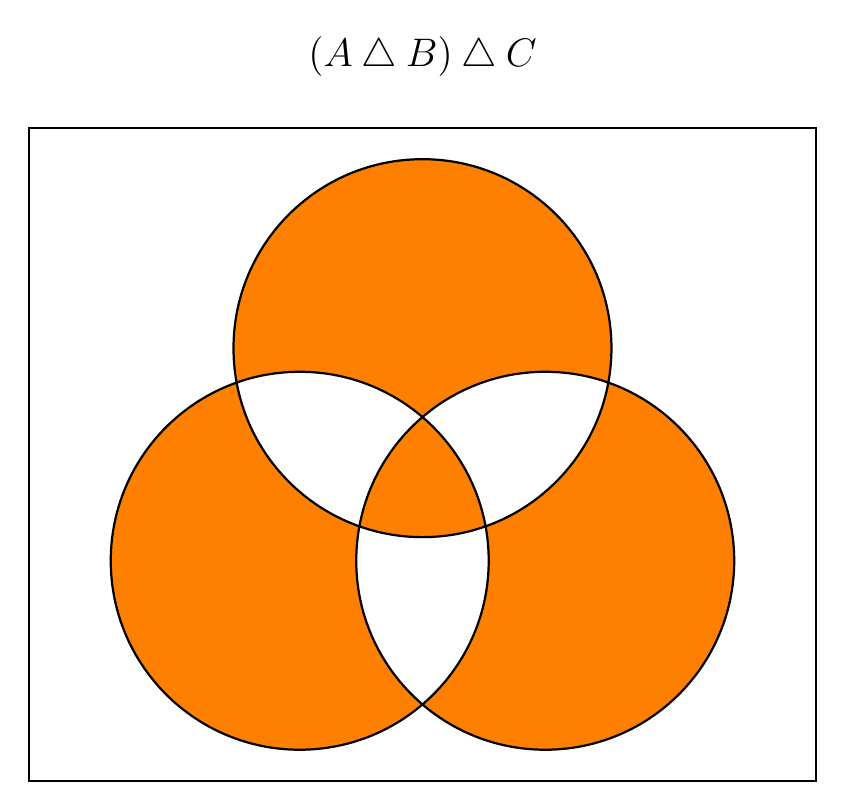
\begin{tikzpicture}
              \def\firstcircle{(90:1.8) circle[radius = 2.4]}
              \def\secondcircle{(210:1.8) circle[radius = 2.4]}
              \def\thirdcircle{(330:1.8) circle[radius = 2.4]}
            
              \draw (0, 5.5) node {\Large $(A \bigtriangleup B) \bigtriangleup C$};
              \draw[thick] (-5, -3.7) rectangle (5, 4.6);
            
              \fill[even odd rule, orange] \firstcircle \secondcircle \thirdcircle;
              \draw[thick] \firstcircle \secondcircle \thirdcircle;
            
              %\node[fill = white, shape = circle] (0,0);
              % Reference used: https://tex.stackexchange.com/questions/329371/how-i-draw-the-symmetrical-difference-of-three-sets-with-venn-diagrams-using-tik
            \end{tikzpicture}

       
    \end{solution}

  \part[5] Using the insights from above, express $A\oplus B\oplus C$ in the same manner as given in part a). That is, using the basic set operations: union, intersection, and complement. Show your working.
    \begin{solution}
      % Enter your solution here.
      From Q3 part(a), we know that:
      \newline $A\oplus B = (A \union B)-(A \inter B). $
      \newline Therefore, Let the set D be, where 
      \newline $ D = \{ x | $ where x is the symmetric difference of the sets A and B $\}$
      \newline Therefore Equation 1, it can be written as:
      \newline $ D\oplus C = (D \union C) \inter (D \inter C)^{C}.$
      \newline Which leads us to:
      \newline $ D\oplus C = (D \union C) - (D \inter C)$
      \newline As $ D  = (A \union B) - (A \inter B)$, substituting D in Equation 1:
      \newline $A\oplus B\oplus C = (((A \union B) - (A \inter B)) \union C) - (((A \union B) - (A \inter B)) \inter C).$
    \end{solution}

  \end{parts}

\question
  Let $A$ be the set of all numbers that are divisible by 6 and $B$ the set of all numbers that are divisible by $10$.

  \begin{parts}
  \part[5] Write the sets $A$ and $B$ in set notation and describe $A \inter B$ as simply as possible.
    \begin{solution}
      % Enter your solution here.
      Let there be two sets, A and B, where:
      \newline $ A = \{ x | $ where x $\in$ multiples of $6 \}$
      \newline $ B = \{ x | $ where x $\in$ multiples of $10 \}$
      \newline $ A \inter B = \{ X | $ where x $\epsilon$ multiples of $30 \}$
    \end{solution}

  \part[10] Describe the set $A \oplus B$, i.e. the symmetric difference of $A$ and $B$, using set notation. Provide a proof that the set you indicate is indeed the symmetric difference of $A$ and $B$.
    \begin{solution}
      % Enter your solution here.
      Since $ A \oplus B$ means $x \not\in A \inter B$
      \newline It can be also written as through the definition of intersection:
      \newline $ (x \in A \land x\not\in B) \lor (x \not\in A \land x\in B) $
      \newline By the definition of Difference, it can be writted as:
      \newline $ (x \in (A-B)) \lor (x \in (B-A))$
      \newline OR is also referred as Union, so by the definition of Union:
      \newline $ x \in (A-B) \union (B-A)$
      \newline The set $A\oplus B$ is known as a disjunctive union which contains all the elements except the ones 
      that are in both the sets, i.e. intersection. Therefore, $A \oplus B$ will contain all the elements that are divisible by either
      6 or 10 but it will exclude all those elements that will be divisible by both, 6 and 10. 
      \newline $ A\oplus B = \{ x | (x \in x \mod{6} = 0 \land x \not\in \mod{10} = 0) \lor (x \not\in x \mod{6} = 0 \land x \in x \mod{10} = 0 ) \} $ 
    \end{solution}

  \part[5] Given $U = \{x\in \mathbb{N} \mid x \leq 60 \}$, list the elements of $A$, $B$, and $A \oplus B$ 
    \begin{solution}
      % Enter your solution here.
      $ A = \{ 6, 12, 18, 24, 30, 36, 42, 48, 54, 60 \}$
      \newline $ B =  \{ 10, 20, 30, 40, 50, 60 \}$
      \newline $ A \oplus B = \{ 6, 10, 12, 18, 20, 24, 36, 40, 42, 48, 50, 54 \}$
    \end{solution}

  \end{parts}

\question
  Show that $\overline{ A \union \overline{B}} = \overline{A} \inter B$.
  \begin{parts}
    
  \part[5] by using set identities.
    \begin{solution}
      % Enter your solution here.
      \newline Applying De Morgan's Law:
      \newline $ A^{C} \inter (B^{C})^{C}$
      \newline Applying Complement Law:
      \newline $ A^{C} \inter B  $
    \end{solution}
    
  \part[5] by proving that each set is a subset of the other.
    \begin{solution}
      % Enter your solution here.
      \newline By approaching the Left Hand Side
      \newline $ \{ x | x \not\in (A \union B^{C}) \}$
      \newline Applying De Morgan's Law:
      \newline $ \{ x | (x \not\in A) \land (x \not\in B^{C}) \}$
      \newline $ \{ x | (x \in A^{C}) \land (x \in B) \}$
      \newline $(A^{C} \inter B)$
      \newline
      \newline Now, by approaching the Right Hand Side
      \newline $A^{C} \inter B$
      \newline $\{ x | x \not\in (A \inter B^{C})$
      \newline $\{ x | x \not\in A \land x\not\in B$
      \newline Complement Law applied
      \newline $A^{C} \inter B$
      \newline Applying De Morgan's Law:
      \newline $(A^{C} \union B^{C})^{C} $
      \newline Therefore, since Right Hand Side and Left Hand Side is proved. Each set is a subset of another

    \end{solution}

  \end{parts}
\end{questions}

1) Venn Diagram help taken by: https://tex.stackexchange.com/questions/329371/how-i-draw-the-symmetrical-difference-of-three-sets-with-venn-diagrams-using-tik


\end{document}

%%% Local Variables:
%%% mode: latex
%%% TeX-master: t
%%% End:
